\chapter*{Anhang}
% =================================================================
\thispagestyle{fancy} \addcontentsline{toc}{chapter}{Anhang}
% =================================================================
\section{Messresultate}
\begin{figure}[h]
\centering
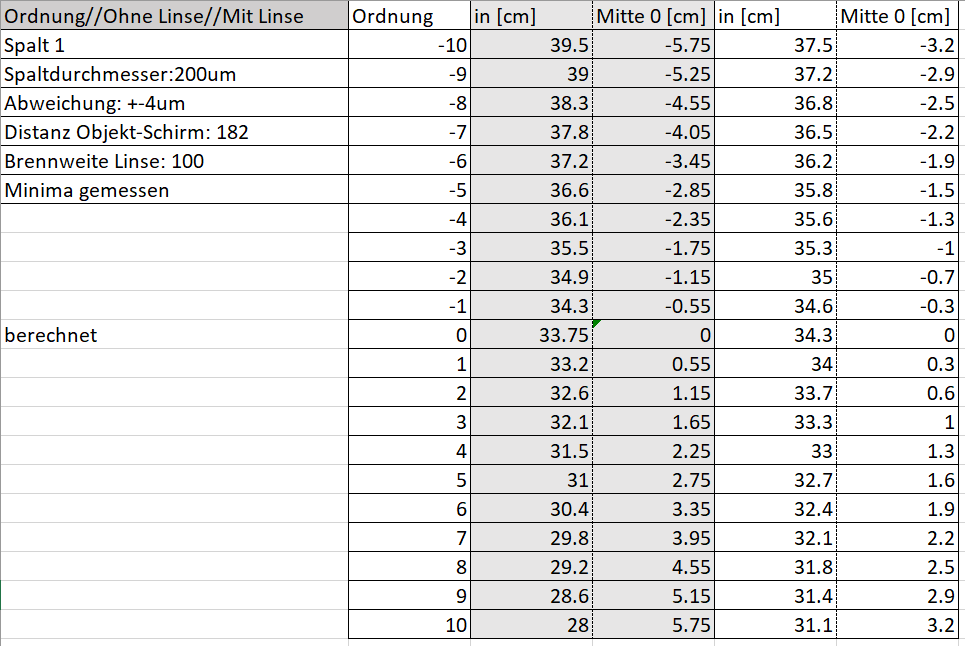
\includegraphics[width=\textwidth]{Bilder/messung1.png} 
\label{fig:messresultate}
\caption{Messresultate Spalt 1}
\end{figure}
\newpage

\begin{figure}[h]
\centering
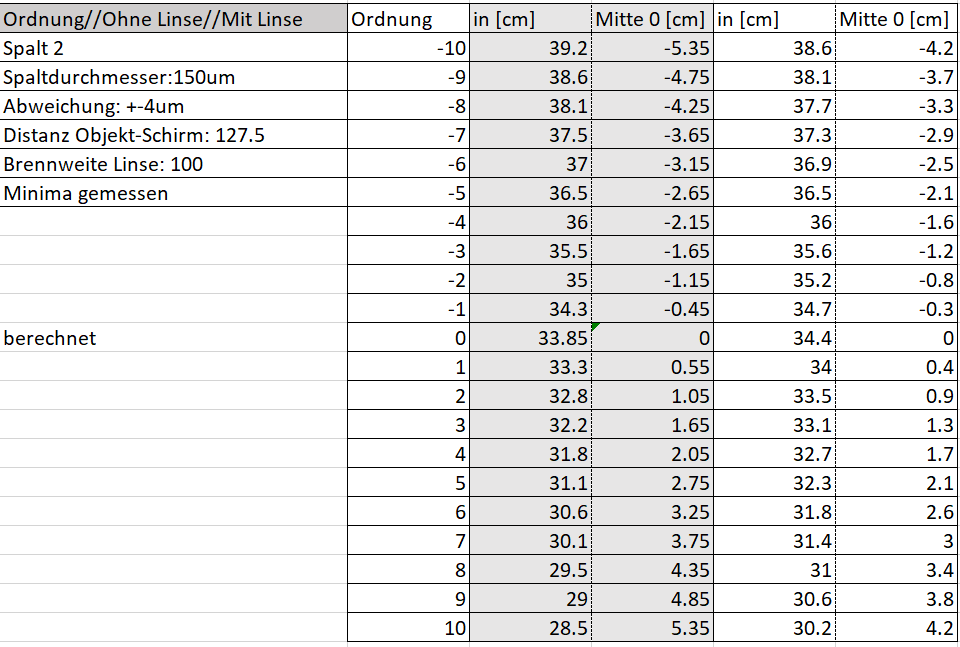
\includegraphics[width=\textwidth]{Bilder/messung2.png} 
\label{fig:messresultate}
\caption{Messresultate Spalt 2}
\end{figure}
\newpage

\begin{figure}[h]
\centering
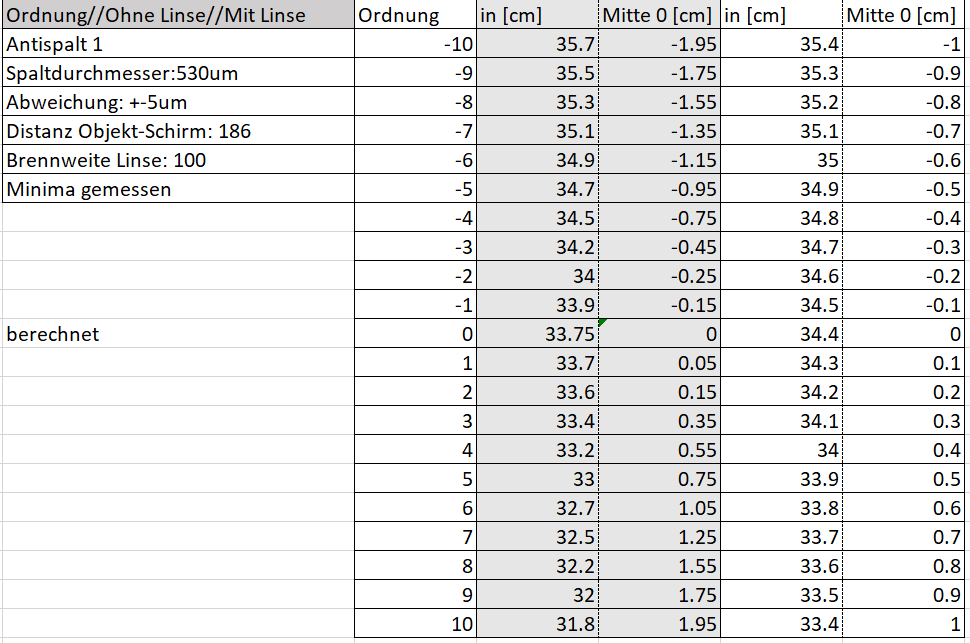
\includegraphics[width=\textwidth]{Bilder/messung3.png} 
\label{fig:messresultate}
\caption{Messresultate Antispalt 1}
\end{figure}
\newpage

\begin{figure}[h]
\centering
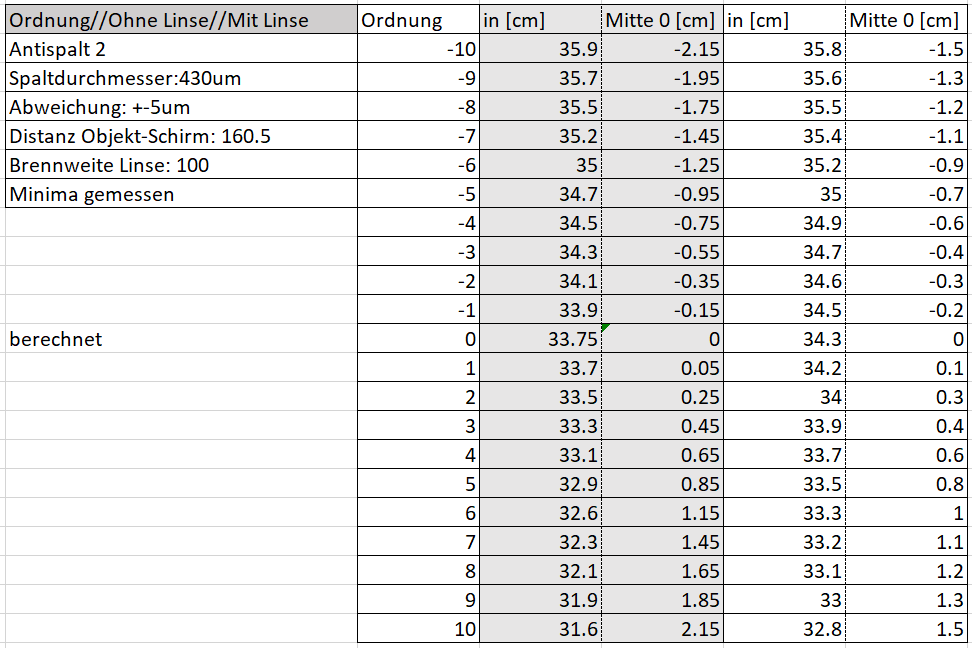
\includegraphics[width=\textwidth]{Bilder/messung4.png} 
\label{fig:messresultate}
\caption{Messresultate Antispalt 2}
\end{figure}
\newpage

\begin{figure}[h]
\centering
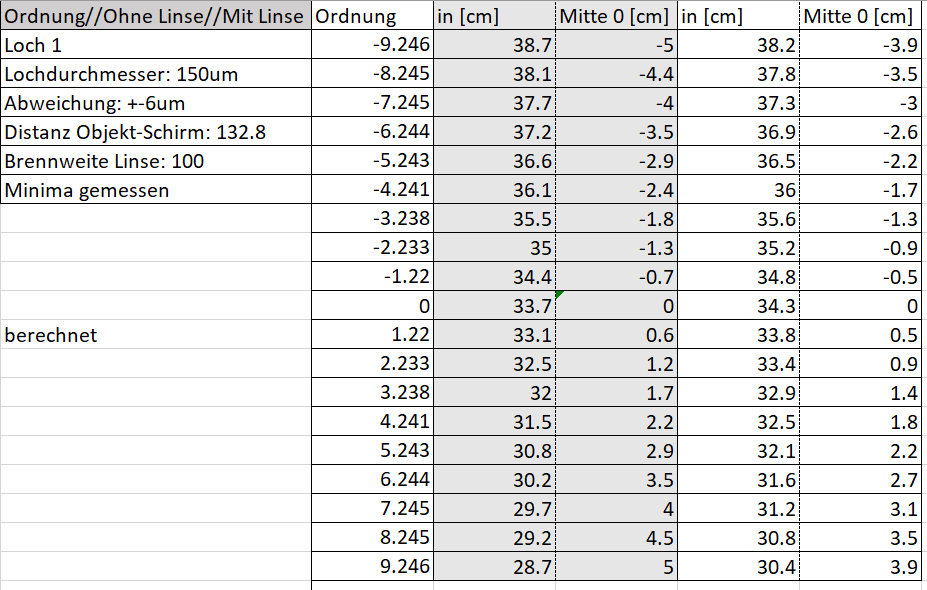
\includegraphics[width=\textwidth]{Bilder/messung5.png} 
\label{fig:messresultate}
\caption{Messresultate Loch 1}
\end{figure}
\newpage

\begin{figure}[h]
\centering
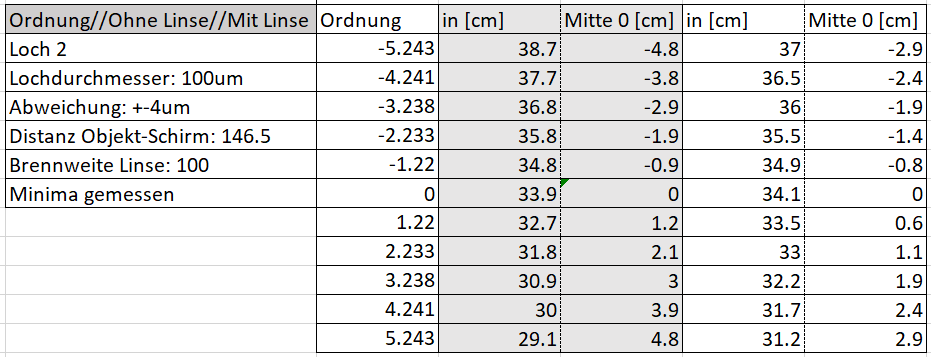
\includegraphics[width=\textwidth]{Bilder/messung6.png} 
\label{fig:messresultate}
\caption{Messresultate Loch 2}
\end{figure}
\newpage

\begin{figure}[h]
\centering
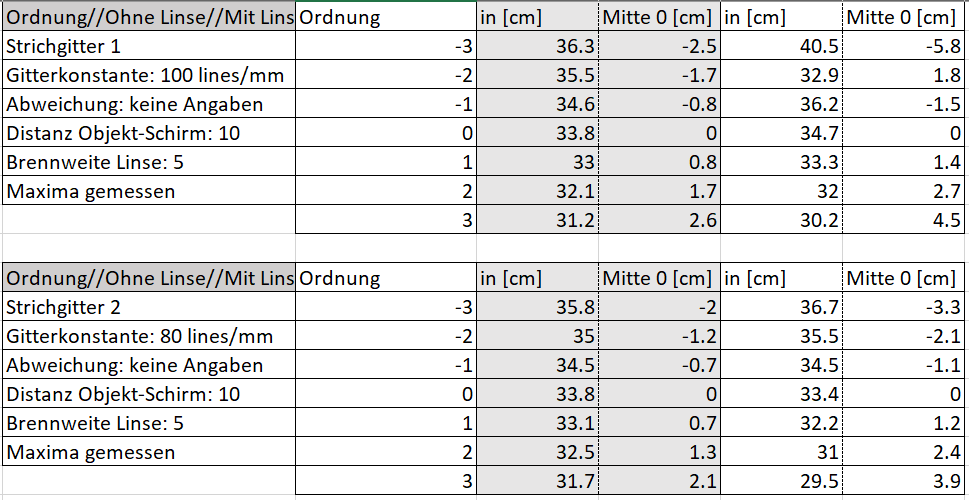
\includegraphics[width=\textwidth]{Bilder/messung7.png} 
\label{fig:messresultate}
\caption{Messresultate Strichgitter 1\&2}
\end{figure}
\newpage

\section{Beugung am Strichgitter}
\label{sec:BeugungAmStrichgitter} \zlabel{sec:BeugungAmStrichgitter}
Auf dem Schirm wurden in diesem Teilversuch die Maximas des Interferenzmusters gemessen und mittels QTI-Plot graphisch dargestellt. Dabei wurden die Gitterlinienabstände mittels der Gleichung \ref{eq:1} ermittelt.

\begin{figure}[h]
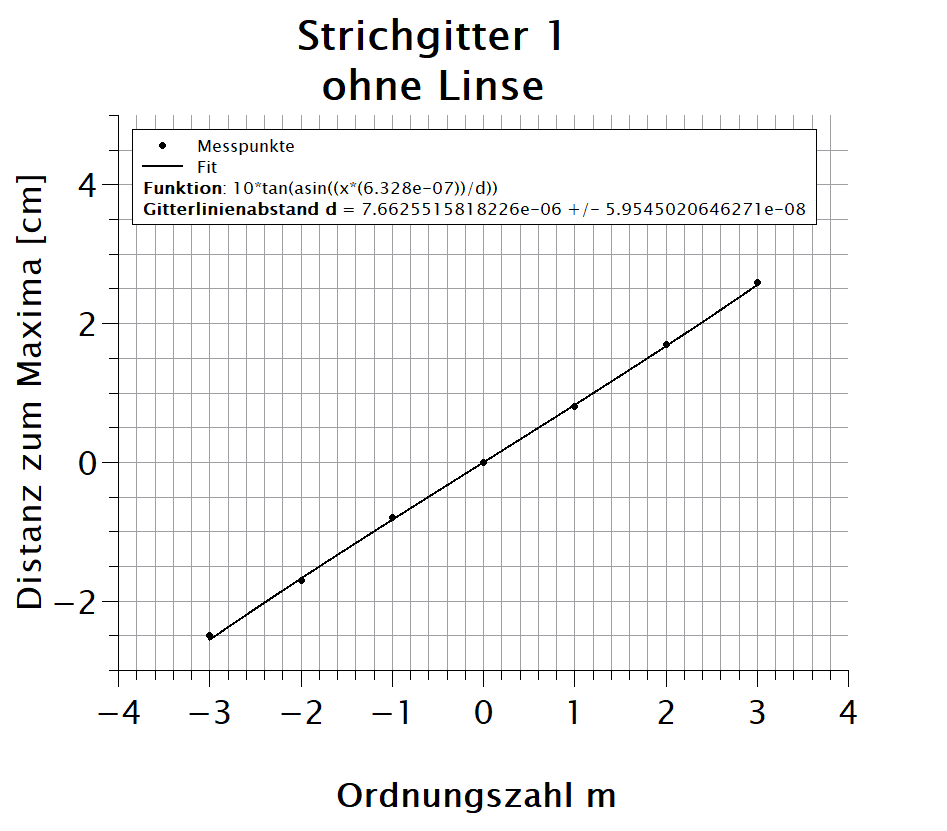
\includegraphics[width=\textwidth]{Bilder/strichgitter1_ohneLinse.png} 
\caption[Strichgitter 1: ohne Linse]{Die Abstände vom Nullpunkt zu den Maximas des Interferenzmusters bei direkter Betrachtung und ohne Linse sind hier graphisch dargestellt. Hier wurde direkt in die Formel \ref{eq:1} der Abstand vom Strichgitter zum Schirm von 10cm eingetragen.}
\label{fig:strichgitter1_ohneLinse}
\end{figure}
\newpage
\begin{figure}[h]
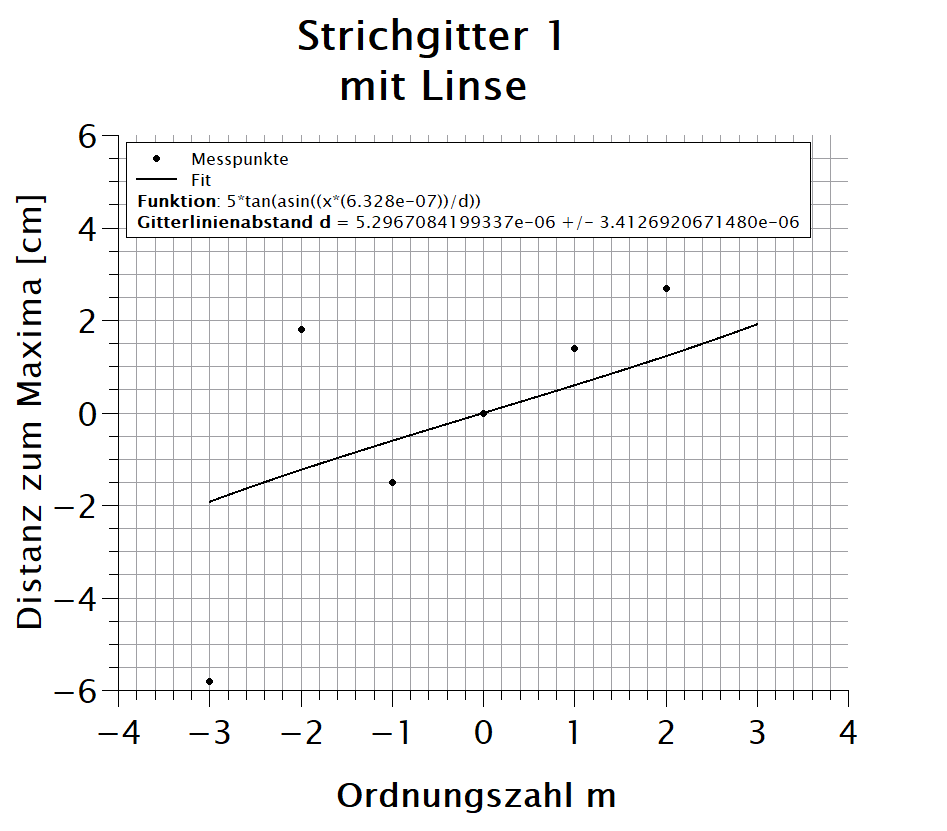
\includegraphics[width=\textwidth]{Bilder/strichgitter1_mitLinse.png} 
\caption[Strichgitter 1: mit Linse]{Die Abstände vom Nullpunkt zu den Maximas des Interferenzmusters bei Frauenhofer'scher Betrachtung und ohne Linse sind hier graphisch dargestellt. Hier wurde direkt in die Formel \ref{eq:1} der Abstand von der Linse zum Schirm von 5cm eingetragen.}
\label{fig:strichgitter1_mitLinse}
\end{figure}
\newpage

\begin{figure}[h]
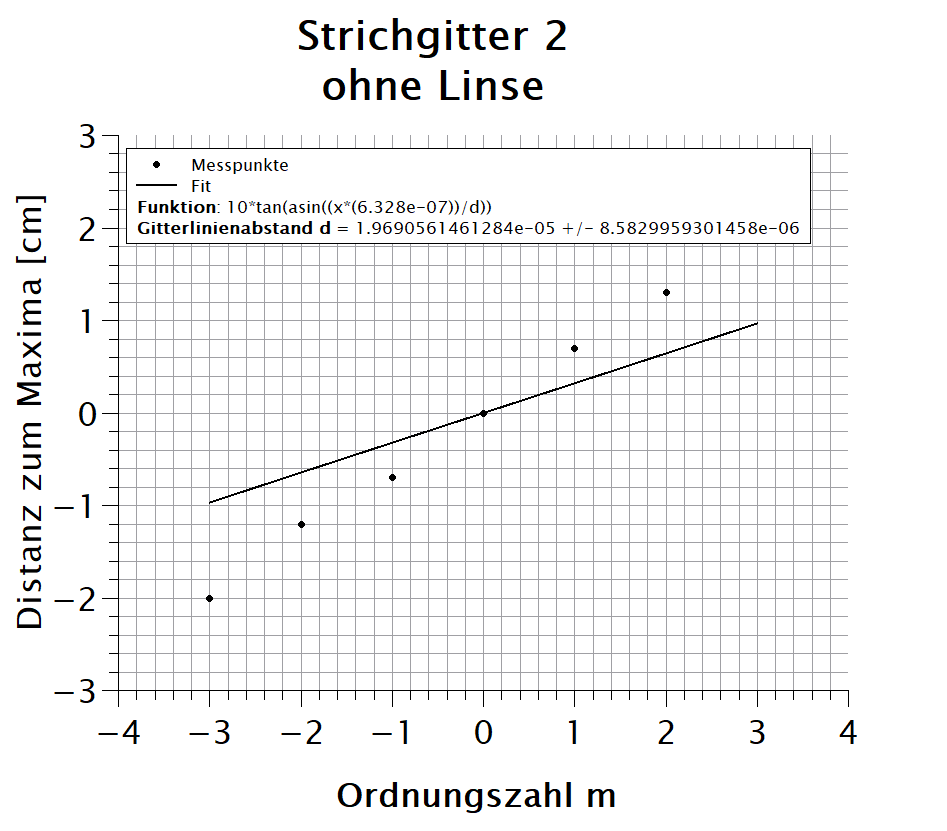
\includegraphics[width=\textwidth]{Bilder/strichgitter2_ohneLinse.png} 
\caption[Strichgitter 2: ohne Linse]{Die Abstände vom Nullpunkt zu den Maximas des Interferenzmusters bei direkter Betrachtung und ohne Linse sind hier graphisch dargestellt. Hier wurde direkt in die Formel \ref{eq:1} der Abstand vom Strichgitter zum Schirm von 10cm eingetragen.}
\label{fig:strichgitter2_ohneLinse}
\end{figure}
\newpage
\begin{figure}[h]
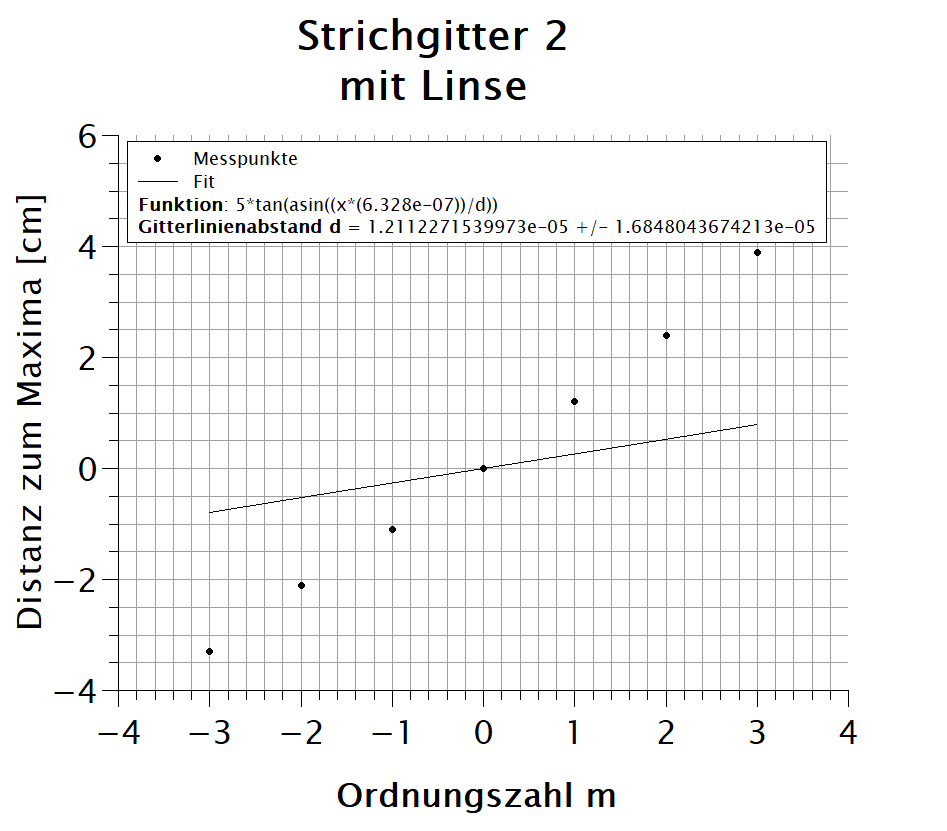
\includegraphics[width=\textwidth]{Bilder/strichgitter2_mitLinse.png} 
\caption[Strichgitter 2: mit Linse]{Die Abstände vom Nullpunkt zu den Maximas des Interferenzmusters bei Frauenhofer'scher Betrachtung und ohne Linse sind hier graphisch dargestellt. Hier wurde direkt in die Formel \ref{eq:1} der Abstand von der Linse zum Schirm von 5cm eingetragen.}
\label{fig:strichgitter1_mitLinse}
\end{figure}
\newpage